\documentclass{standalone}
\usepackage{tikz}
\usepackage{ctex,siunitx}
\setCJKmainfont{Noto Serif CJK SC}
\usepackage{tkz-euclide}
\usepackage{amsmath,upgreek}
\usetikzlibrary{patterns, calc,3d}
\usetikzlibrary {decorations.pathmorphing,decorations.pathreplacing,decorations.shapes}
\begin{document}
\small
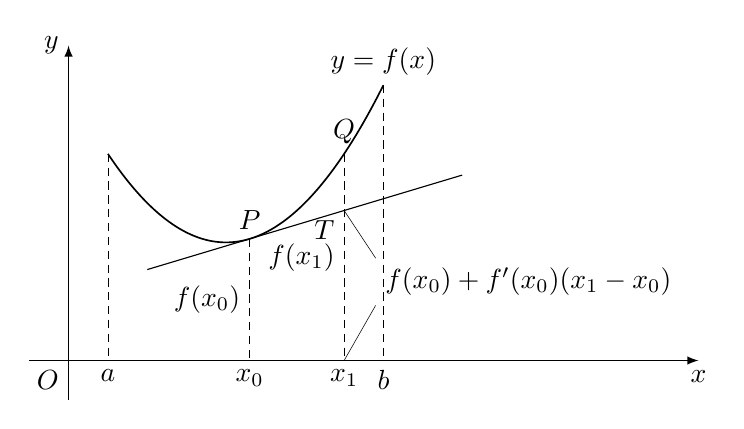
\begin{tikzpicture}[>=latex,scale=1.0]
  \draw[->](-0.5,0)--(8,0)node[below]{$x$};
  \draw[->](0,-0.5)--(0,4)node[left]{$y$};
  \node at (0,0)[below left]{$O$};
  \draw[samples=200,domain=0.5:4,semithick]plot(\x,{0.5*\x*\x-2*\x+3.5})node[above]{$y=f(x)$};
  \draw[very thin,densely dashed](0.5,2.625)--(0.5,0)node[below]{$a$};
  \draw[very thin,densely dashed](4,3.5)--(4,0)node[below]{$b$};
  \draw[very thin,densely dashed](2.3,1.545)node[above]{$P$}--(2.3,0)node[below]{$x_0$}node[midway,left]{$f(x_0)$};
  \draw[very thin,densely dashed](3.5,2.625)node[above]{$Q$}--(3.5,0)node[below]{$x_1$}node[midway,left]{$f(x_1)$};
  \draw(1.0,1.155)--++(4,1.2);
  \node at (3.5,1.905)[below left]{$T$};
  \node (eq) at (3.9,1.0)[right]{$f(x_0)+f'(x_0)(x_1-x_0)$};
  \draw[very thin](3.5,1.905)--(eq.north west)(3.5,0)--(eq.south west);
  % \draw[densely dashed](0,-1)--(3,-1)--(3,0)node[above]{3};
  % \draw[densely dashed](0,3)node[left]{3}--(1,3)--(1,0)node[below]{1};
  % \draw[densely dashed](0,1)node[left]{1}--(2,1)--(2,0)node[below]{2};
  % \draw(0.1,2)--(0,2)node[left]{2};
\end{tikzpicture}
\end{document}